%\definecolor{customgreen}{HTML}{82B366}
%\definecolor{customblue}{HTML}{6C8EBF}

%\def\svgwidth{\textwidth}
%\includesvg[inkscapelatex=true]{figs/Diagram2}
% \centering
% \caption{Diagram caption}
% \label{fig:teaser}
% Add the legend below the diagram
%\begin{tikzpicture}
%    % Green square for "Choose one"
%    \node[fill=customgreen, minimum size=10pt, anchor=west] (green) at (0, 0) {};
%    \node[anchor=west] at (0.3, 0) {Choose one path};

    % Blue square for "Need all paths"
%    \node[fill=customblue, minimum size=10pt, anchor=west] (blue) at (0, -0.6) {};
%    \node[anchor=west] at (0.3, -0.6) {Need all paths};
%  \end{tikzpicture}

\usetikzlibrary{arrows.meta, positioning}
\centering
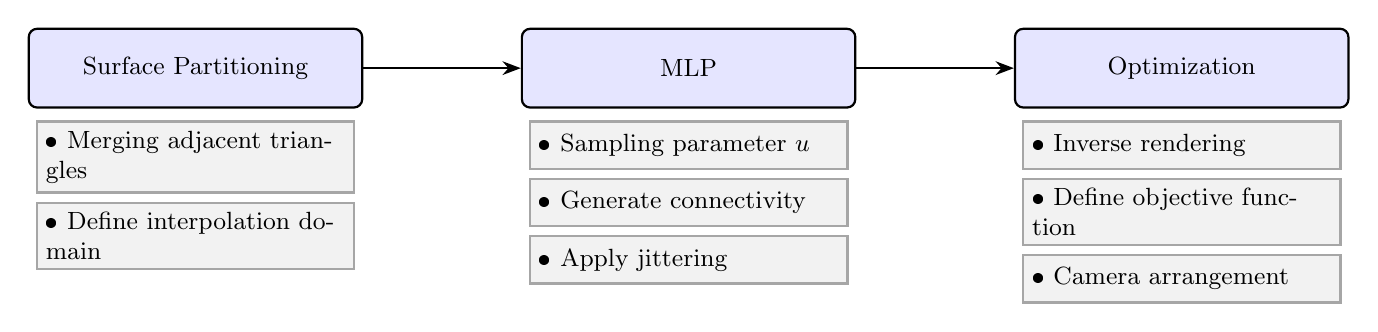
\begin{tikzpicture}[
  node distance=0.8cm and 2cm,
  font=\small,
  stage/.style={
    rectangle, rounded corners=3pt, draw=black, thick,
    text width=4cm, minimum height=1cm, align=center, fill=blue!10
  },
  substep/.style={
    rectangle, draw=gray!70, thick, text width=3.8cm,
    minimum height=0.6cm, align=left, fill=gray!10
  },
  arrow/.style={thick, ->, >=Stealth}
]

% Stage 1
\node (stage1) [stage] {Surface Partitioning};
\node (s1a) [substep, below=0.15cm of stage1] {• Merging adjacent triangles};
\node (s1b) [substep, below=0.1cm of s1a] {• Define interpolation domain};

% Stage 2
\node (stage2) [stage, right=of stage1] {MLP};
\node (s2a) [substep, below=0.15cm of stage2] {• Sampling parameter $u$};
\node (s2b) [substep, below=0.1cm of s2a] {• Generate connectivity};
\node (s2c) [substep, below=0.1cm of s2b] {• Apply jittering};

% Stage 3
\node (stage3) [stage, right=of stage2] {Optimization};
\node (s3a) [substep, below=0.15cm of stage3] {• Inverse rendering};
\node (s3b) [substep, below=0.1cm of s3a] {• Define objective function};
\node (s3c) [substep, below=0.1cm of s3b] {• Camera arrangement};

% Arrows
\draw [arrow] (stage1) -- (stage2);
\draw [arrow] (stage2) -- (stage3);

\end{tikzpicture}
\vspace{-0.5em}
\caption{Overview of the proposed method: Surface Partitioning, followed by MLP-based modeling, and final optimization via inverse rendering.}
\label{fig:teaser}